% French labels; written by tools/paper-figures.py from ranges.tex.
% The national ranges of two names, from model/areas/name-blocks.csv.
% Written by tools/paper-figures.py; do not edit by hand.
\documentclass[tikz,border=2mm]{standalone}
\usepackage{fontspec}\setmainfont{LibertinusSans}[Extension=.otf,UprightFont=*-Regular,BoldFont=*-Bold]
\usetikzlibrary{patterns}
\definecolor{blk}{HTML}{009E60}
\definecolor{tail}{HTML}{8FD3B4}
\begin{document}
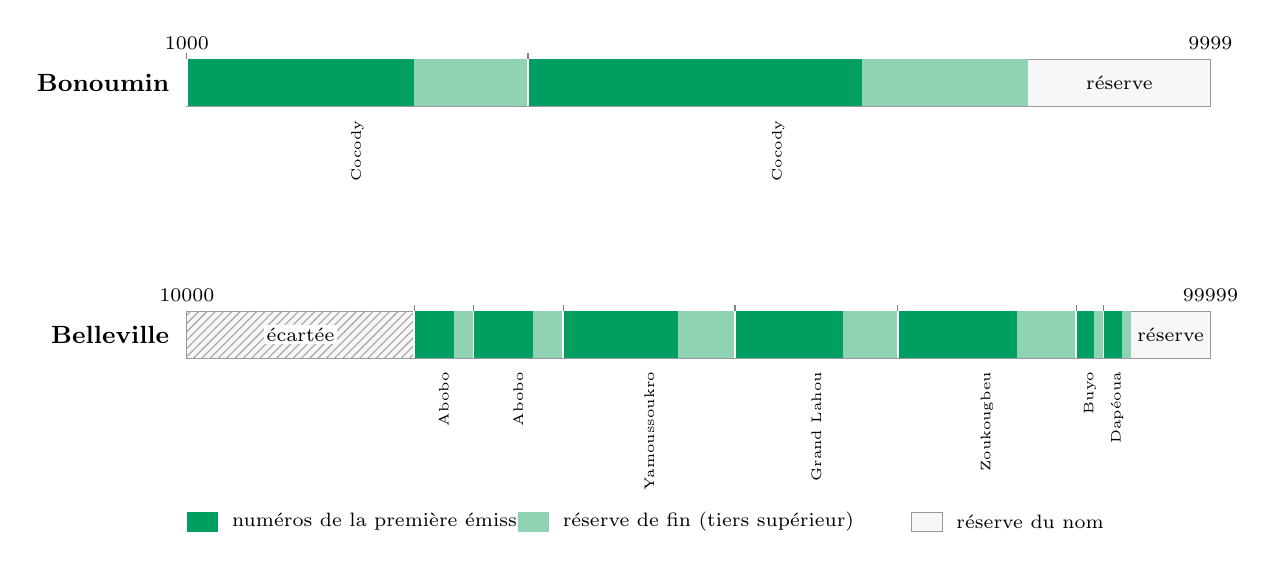
\begin{tikzpicture}
\node[left,font=\small\bfseries] at (-0.1,3.50) {Bonoumin};
\draw[black!40,line width=0.3pt,fill=black!3] (0,3.20) rectangle (13.000,3.80);
\fill[blk] (0.000,3.20) rectangle (2.889,3.80);
\fill[tail] (2.889,3.20) rectangle (4.333,3.80);
\draw[white,line width=0.6pt] (0.000,3.20) -- (0.000,3.80);
\node[font=\tiny,rotate=90,anchor=east] at (2.167,3.15) {Cocody};
\fill[blk] (4.333,3.20) rectangle (8.570,3.80);
\fill[tail] (8.570,3.20) rectangle (10.689,3.80);
\draw[white,line width=0.6pt] (4.333,3.20) -- (4.333,3.80);
\node[font=\tiny,rotate=90,anchor=east] at (7.511,3.15) {Cocody};
\node[font=\scriptsize] at (11.844,3.50) {réserve};
\node[font=\scriptsize,above] at (0.000,3.80) {1000};
\node[font=\scriptsize,above] at (13.000,3.80) {9999};
\draw[black!50] (0.000,3.80) -- ++(0,0.08);
\draw[black!50] (4.333,3.80) -- ++(0,0.08);
\node[left,font=\small\bfseries] at (-0.1,0.30) {Belleville};
\draw[black!40,line width=0.3pt,fill=black!3] (0,0.00) rectangle (13.000,0.60);
\fill[pattern=north east lines,pattern color=black!35] (0.000,0.00) rectangle (2.889,0.60);
\node[font=\scriptsize,fill=white,inner sep=1pt] at (1.444,0.30) {écartée};
\fill[blk] (2.889,0.00) rectangle (3.390,0.60);
\fill[tail] (3.390,0.00) rectangle (3.640,0.60);
\draw[white,line width=0.6pt] (2.889,0.00) -- (2.889,0.60);
\node[font=\tiny,rotate=90,anchor=east] at (3.264,-0.05) {Abobo};
\fill[blk] (3.640,0.00) rectangle (4.401,0.60);
\fill[tail] (4.401,0.00) rectangle (4.781,0.60);
\draw[white,line width=0.6pt] (3.640,0.00) -- (3.640,0.60);
\node[font=\tiny,rotate=90,anchor=east] at (4.211,-0.05) {Abobo};
\fill[blk] (4.781,0.00) rectangle (6.235,0.60);
\fill[tail] (6.235,0.00) rectangle (6.962,0.60);
\draw[white,line width=0.6pt] (4.781,0.00) -- (4.781,0.60);
\node[font=\tiny,rotate=90,anchor=east] at (5.872,-0.05) {Yamoussoukro};
\fill[blk] (6.962,0.00) rectangle (8.339,0.60);
\fill[tail] (8.339,0.00) rectangle (9.028,0.60);
\draw[white,line width=0.6pt] (6.962,0.00) -- (6.962,0.60);
\node[font=\tiny,rotate=90,anchor=east] at (7.995,-0.05) {Grand Lahou};
\fill[blk] (9.028,0.00) rectangle (10.540,0.60);
\fill[tail] (10.540,0.00) rectangle (11.296,0.60);
\draw[white,line width=0.6pt] (9.028,0.00) -- (9.028,0.60);
\node[font=\tiny,rotate=90,anchor=east] at (10.162,-0.05) {Zoukougbeu};
\fill[blk] (11.296,0.00) rectangle (11.527,0.60);
\fill[tail] (11.527,0.00) rectangle (11.642,0.60);
\draw[white,line width=0.6pt] (11.296,0.00) -- (11.296,0.60);
\node[font=\tiny,rotate=90,anchor=east] at (11.469,-0.05) {Buyo};
\fill[blk] (11.642,0.00) rectangle (11.873,0.60);
\fill[tail] (11.873,0.00) rectangle (11.989,0.60);
\draw[white,line width=0.6pt] (11.642,0.00) -- (11.642,0.60);
\node[font=\tiny,rotate=90,anchor=east] at (11.816,-0.05) {Dapéoua};
\node[font=\scriptsize] at (12.494,0.30) {réserve};
\node[font=\scriptsize,above] at (0.000,0.60) {10000};
\node[font=\scriptsize,above] at (13.000,0.60) {99999};
\draw[black!50] (2.889,0.60) -- ++(0,0.08);
\draw[black!50] (3.640,0.60) -- ++(0,0.08);
\draw[black!50] (4.781,0.60) -- ++(0,0.08);
\draw[black!50] (6.962,0.60) -- ++(0,0.08);
\draw[black!50] (9.028,0.60) -- ++(0,0.08);
\draw[black!50] (11.296,0.60) -- ++(0,0.08);
\draw[black!50] (11.642,0.60) -- ++(0,0.08);
\fill[blk] (0,-2.2) rectangle (0.4,-1.95); \node[right,font=\scriptsize] at (0.45,-2.075) {numéros de la première émission};\fill[tail] (4.2,-2.2) rectangle (4.6,-1.95); \node[right,font=\scriptsize] at (4.65,-2.075) {réserve de fin (tiers supérieur)};\fill[black!3,draw=black!40,line width=0.3pt] (9.2,-2.2) rectangle (9.6,-1.95); \node[right,font=\scriptsize] at (9.65,-2.075) {réserve du nom};
\end{tikzpicture}
\end{document}
